\chapter{Self-Healing Classification Schema} \label{ch:SelfHealingClassificationSchema}



\textbf{3.1. Domain:\\}
The surveyed literature has been classified by discussing the self-healing techniques that has been designed and implemented in the several applications areas. The different approaches are summarized in table 1.In each of the cases the table describes the self-healing approach and the techniques that has been used in each of the stages of the self-healing loops for detecting, diagnosing and recovering.
\cite{Harald:SelfHealingSurvey:2011}.\\

\begin{center}
    \begin{tabular}{ | p{3cm} | p{11cm} |}
    \hline
    Research Area & Summary \\ \hline
    Embedded Systems & Embedded systems are computer systems that are part of larger
systems and performs some of the requirements of these systems. Examples of such systems are auto mobile control systems, industrial processes control systems, mobile phones, or small sensor controllers. 
New ideas begin self-healing approaches to define recovery techniques focusing on the whole system instead of focusing on the recovery of individual components.
\cite{Harald:SelfHealingSurvey:2011}.
\cite{Crnkovic:SelfHealingSurvey:2005}.\\

\\ \hline
    Operating Systems & An operating system (OS) is a collection of software that allows a user or programmer to make use of the underlying hardware easier.New ideas begin a self-healing manager which keeps a track of the failures and re-runs the stopped services.
    
 \\ \hline
    Architecture Based & An Architecture- Based System is a conceptual model that defines the structure of a system. A system architecture is described using Architecture Description Languages (ADLs).New ideas begin with the help of architectural models expressed by architectural description language (ADL) differences between runtime composition and healthy model of composition are identified. \\
    \hline
    Cross/Multi-Layer-Base & A multi-layered software architecture is a software architecture that uses many layers for allocating the different responsibilities of a software product. New ideas begin with organizing the resources into layers. One approach uses the layers to avoid conflicts in resource allocation and other resource boundary and priorities.  \\ \hline
        Multi Agent-based & Multi-agent systems are distributed computing systems, that are composed of a number of interacting computational entities.New ideas begin in Agent-based environments act autonomously and host self-healing capabilities that protects the system part. 
 \\ \hline
     Reflective-middle-ware & New ideas begin on self-healing techniques on the middleware. This approach combines the properties of reflective middleware to self-healing enhancement.
 \\ \hline
      Legacy application and AOP & New ideas begin on self-healing techniques. The idea begins with finding checkpoints for monitoring recovery actions. This feature is provided by linker, runtime for legacy applications or implemented by aspect-oriented programming.
 \\ \hline
  Discovery systems and AOP & A discovery system is an artificial intelligence system which attempts to discover new scientific concepts or laws.
They are designed to support the discovery of different resources distinct requirements specified by individual semantics. New ideas begin that instead of deploying recovery strategy, try to keep request latency minimum and query responses consistent.
  \\ \hline
   Web services and QoS-based and AOP & New ideas begin with combining the monitoring and recovery capabilities to a self-healing loop. 
    \end{tabular}
\end{center}





\textbf{3.2. Technical Approach:\\}

Novel research ideas on Self-Healing Techniques\\

Some of the recent emergence of novel research ideas which addresses the issue of recovery in the presence of faults more efficiently are as follows. Amongst the below mentioned techniques: Failure-Oblivious Computing and Error Virtualization are termed as continued execution and are more highly valued than absolute correctness techniques (The method mentioned above)
\cite{Keromytis:SelfHealingSurvey:2011}.\\

\textit{3.2.1.Failure-Oblivious Computing:}
Failure oblivious computing mainly handles memory errors. In this technique the program code is extensively written to check for every memory access.
Failure-oblivious computing is a strategy that empowers computer programs to keep executing in spite of memory errors. The procedure handles endeavours to read invalid memory by returning back a manufactured value to the program. Thus in this strategy, no endeavour is made to advise the system that an error has occurred\\

\textit{3.2.2.Data-Structure Repair: }
This technique helps in detecting the corrupted data structures and fix it to a match with some pre-defined definitions/factors (Repair Algorithms). The Repair Algorithm produces a Data structure that satisfies consistency properties and is heuristically close to the broken data structure. In most cases it might not be necessary that the same data structure will be produced every time, but the new data structure must have some consistent property and keep the program operating successfully. The most common errors encountered in a Broken Data Structure Are Missing Elements, Inappropriate sharing, Dangling references, Out of bounds array indices and inconsistence values.\\
 
\textit{3.2.3.Error Virtualization: }
The main assumption in error virtualization is that a mapping can be made between the arrangement of set of errors that could happen at the time of program's execution and the restricted arrangement of errors that are explicitly taken care of by the project code.\\ 

By virtualizing the errors, an application can proceed with execution through a fault by invalidating the impacts of such faults and utilizing a manufactured return value for the function where the fault occurred. These return values were dictated by utilizing straightforward heuristics on the return type as controlled by source code analysis.\\

\textit{Smart Error Virtualization (SEV),} is another technique for self-healing that involves learning appropriate function return values at runtime.\\

\textit{3.2.4.Automatic Software Self-Healing Using Error Virtualization Rescue Points (ASSURE)}
ASSURE is an attempt to minize the probability of semantically incorrect response to a fault or attack. ASSURE technique proposes the concept of rescue points. Rescue points induce faults at areas that are known to propagate faults effectively, rather than attempting to mask errors to some previous technologies. The location in the code that handles these sort of anticipated faults leads to safe execution flow. This technique is very similar to exceptional handling that dynamically handles he best scoop to handle an error.\\

\textit{3.2.5.DIRA DIRA:}
DIRA is a technique for automatic detection, identification and repair of control-hijacking attacks. The technique is implemented as a GCC compiler. And uses checkpoints for detecting data structures when they are overwritten.\\

\textit{3.2.6.Vigilante Vigilante:}
This technique helps to detect vulnerability by executing injected code and defines a data-structure to handle this issue. The best part of this technique is that, it is exploit-argostic and is used against polymorphic worms.\\

\textbf{3.3. Steps:\\}

The diagram below shows the different Steps Involved In Survey Of Research In Self-Healing Systems:

\begin{figure}[H]
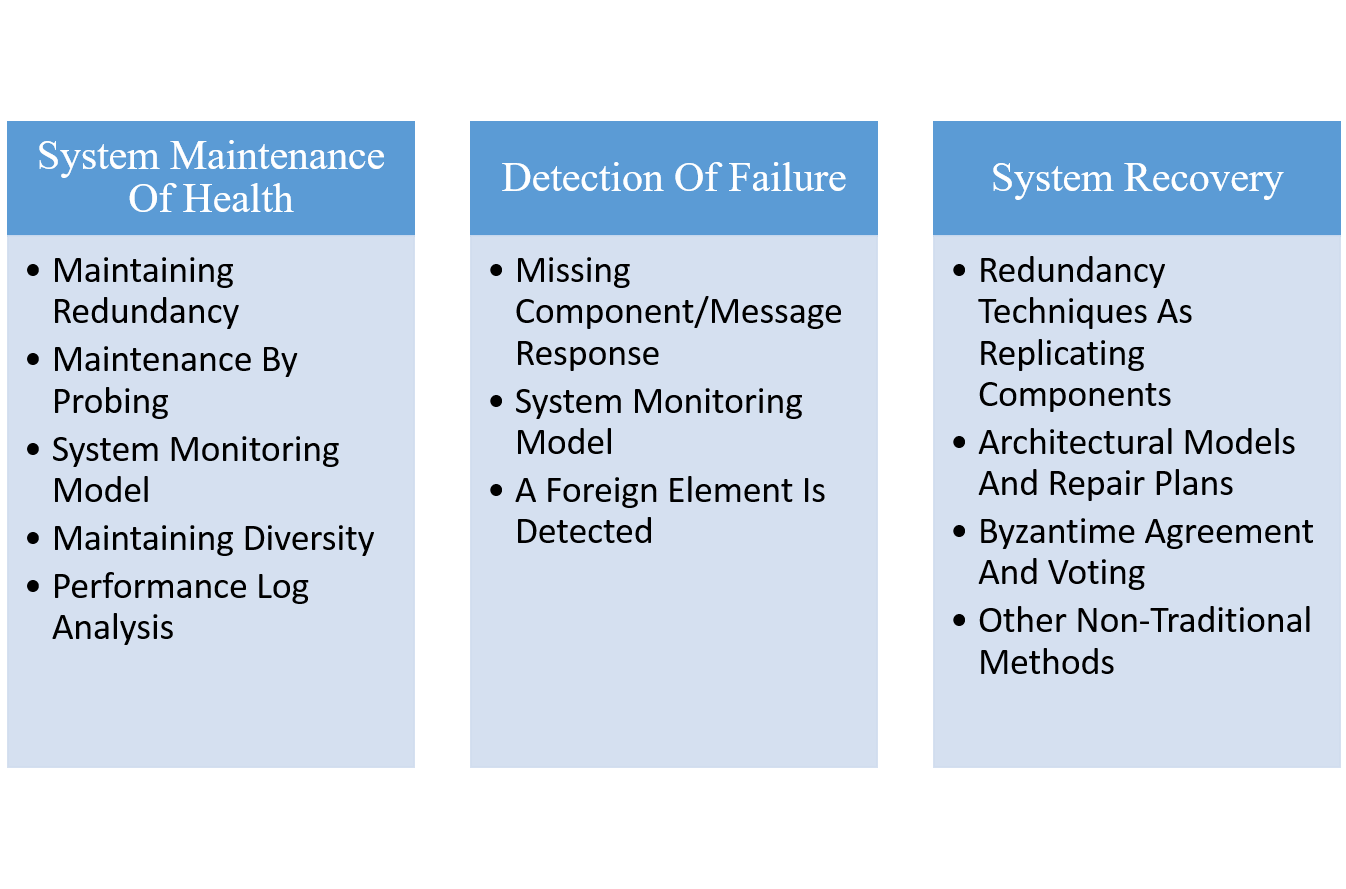
\includegraphics[width=5in]{img/SurveyofSelfHeaingResearch}
\caption{Survey Of Research In Self-Healing Systems:}
\end{figure}



\textbf{\textit{3.3.1.System Maintenance Of Health:}}
System Maintenance Of Health is a mechanism where the system should check for faults periodically to continue monitoring its health.There are various techniques that have been used to maintain the system health are:\\

\textit{1. Maintaining Redundancy:}
Replicating components to maintain redundancy is
always a popular choice in maintaining system health.There are many different redundancy strategies
that researchers in the area of self-healing have pursued.The most promising strategies discussed in this paper are\textit{:Cell Division, Self-Assembly and Multi-Agent Decision Making.}\\

\textit{2. Maintenance By Probing:}
Probing is a mechanism that is commonly used to get
information from the system in order to monitor its health.The different system probing procedures mentioned in the paper are: Grid Adaption/Coordinating SM,Decision And Control Layer,Feedback Control Loop,Adaptive Mirroring, Sensors Gathering Data From Functional Layer.\\

\textit{3. System Monitoring Model:}
Research in the area of self-healing systems includes
literature dealing with architecture models. The literature in this area has been broadly classified into three different categories:
(a) representing the system using Architectural Description Language (ADL), 
(b) representing regularities in a system, 
(c) providing a relational model of the system.\\

\textit{4. Maintaining Diversity:}
Diversity is an important strategy to attain system robustness. The different strategies using system diversity for maintaining system health are: Functionality Based Security, Diverse Design Model, Identify Critical Paths.\\

\textit{5. Performance Log Analysis:}\\
Performance log analysis is a scheme for the analysis of data on performance measures of the system, which can be used for the diagnosis of faults, the detection of intrusion and the facilitation of the healing process. The different strategies using performance log analysis for maintaining system health are: Watchtower, Predict Target Event, Finite Automata Scheme.\\

\textbf{\textit{3.3.2.Detection Of Failure:}}
Failure detection is another major area of research.Several approaches have been adopted
to detect non-self or abnormality in the functioning of the system are:\\

\textit{1. Missing Component/Message Response:}
This subsection discusses the policies where the strategy is to identify something missing from the normal behaviour of the system. Nagpal et al. propose a strategy in which the agents can produce replications when they sense the disappearance of their neighbours. The different strategies, for detecting failure  by sensing something a miss from the regular behaviour of the system are: Disappearance Of Components, Absence Of Message, Missing Response In Query.\\

\textit{2. System Monitoring Model:}
This subsection handles the policies which are suitable for architectures , where the system monitors components by probing.Merideth et al. propose a model in which pro-actively probing a system and collecting a data when a fault is detected improves the survivability of it. The different models for monitoring the system and detecting any failure are Monitoring Data For Trigger,Difference Between Running And Actual System, Parallel Space Servicing, Proactive Probing and Component Addition/Missing\\

\textit{3. A Foreign Element Is Detected:\\}
A proactive containment strategy notifies to the system the presence of a malicious replica.\\

\textbf{\textit{3.3.3.System Recovery:}}
System recovery involves mechanisms to transform a system from an unhealthy state to a healthy state. 
This various redundancy techniques are:\\

\textit{1. Redundancy Techniques As Replicating Components:}

Redundancy is the concept by which system can replicate components to replace dead neighbours and thus can recreate the entire structure.
Regeneration helps in recovering large part of effected system as long as the system has a circle center and enough reference points.The Redundancy techniques for healing are Self-Assembly Of Components, Replicating Cells and Recovery Oriented Computing Research.\\

\textit{2. Architectural Models And Repair Plans:}

In some cases, the Faulty components 
are isolated and the system is reconfigured 
with by incorporating different Repair Plans For Healing. The most important Plans For Healing are Use Of Gauges, Feedback Control Loops, Service and Contract (S+C) Protocol And Event Based Configuration.\\

\textit{3. Byzantine Agreement And Voting:}

For some systems, where the function of the system is to produce output results and the non-faulty components always produce the same value for the output, voting could take place and majority is applied to the output results of all process. In that way, faulty process can be detected and tolerated. (Merideth et al.). Another strategy is to delegate several agents to do the same task, and either select directly or vote on the agent that achieves the best complexity (on time, space, etc.) (Huhns et al).\\

\textit{4. Other Non-Traditional Methods}

Some Of the other non-traditional approaches used for system recovery are The Recovery-Oriented Computing Research Used at UC Berkley/Stanford and Failure Reporting Methodologies Used By The PSTN (public switched telephone network). 

\cite{Ghosh:SelfHealingSurvey:2007}.\\








